\documentclass{article}

\usepackage[polish]{babel}
\usepackage[T1]{fontenc}
\usepackage[utf8]{inputenc}
%\usepackage{txfonts}
\usepackage{amsmath}
\usepackage{listings}
\usepackage{graphicx}

\title{Aukcje kombinatoryczne}
\author{Piotr Rzepecki, Krzysztof Zielonka}

\date{\today}

\begin{document}

\maketitle

\section{Wstęp}
\begin{frame}{Opis problemu}
    \begin{block}{Aukcje kombinatoryczne}
        W aukcjach kombinatorycznych (ang.combinatorialauc-tion) przedmiotem handlu jest wiele towarów. Uczestnicy mogą składać oferty na zbiory towarów i te oferty s ą nie-podzielne, tzn. muszą być przyjęte w całości lub w całości odrzucone. Problem wyznaczania zbioru ofert przyjętych maksymalizujących przychódw takiej aukcji jest w ogólnym przypadku NP -trudnym problemem kombinatorycznym.
    \end{block}
    % http://www.academia.edu/395279/ALGORYTMY_PRZYBLIZONEGO_ROZWI_AZYWANIA_PROBLEMU_AUKCJI_KOMBINATORYCZNEJ
\end{frame}

\begin{frame}{Representacja danych i rozwiązania}

    \begin{block}{Reprezentacja danych}
        Dane to liczba towarów $n$ i $m$ ofert, gdzie każda oferta to lista towarów i proponowana za nie cena.
    \end{block}

    \begin{block}{Reprezentajca rozwiązania}
        Permutacja ofert, którą rozumiemy jako kolejność rozpatrywania ofert.
        Oferta jest przyjmowana jeśli żaden z jej towarów nie został już wykupiony przez jakąs wcześniejszą ofertę.
    \end{block}

    \begin{block}{Funkcja celu}
        Akceptujemy oferty w kolejności występowania ich identyfikatorów w permutacji i wybierajać te, których towary są jeszcze dostępne.
        Jako wartość celu przyjmujemy sume cen zaakceptowanych ofert.
        %\begin{equation}
        %    f(x) = \sum\limits_{i=1}^{m} o_{m,1}
        %\end{equation}
    \end{block}
\end{frame}

\begin{frame}{Rozwiązanie problemu}
    \begin{itemize}
        \item Do rozwiązania problemu wykorzystujemy algorytm SGA.
        \item Operator krzyżowania to lekko zmodyfikowany operaotr PMX (staramy sie aby wymieniane środkowe segenty były częściej wybierane z lewej storny osobnika niz prawej).
        \item Operator mutacji przesuwa całą permutacje o jeden element w lewo.
    \end{itemize}
\end{frame}

\begin{frame}{Dane testowe}
    Do generowania danych testów korzystamy z generatora stworzonego przez bla bla.
\end{frame}




\section{Rozwiązanie przy użycia wektora binarnego}
\subsection{Reprezentacja rozwiązania}

Reprezentacja za pomocą wektora binarnego w której jedynkę interpretujemy jako ofertę możliwą do zaakceptowania, a zero za jej definitywne odrzucenie. W szczególności, wartość 1 nie oznacza, że oferta zostanie zaakceptowana ze względu na możliwy konflikt z inną ofertą (dzięki temu zyskujemy to, że każdy osobnik w populacji koduje poprawne rozwiązanie).

Taka reprezentacja pozwoliła nam zastosować algorytm PBIL do rozwiązania tego problemu.

\subsection{Funkcja celu}
Funkcja celu analizuje wektor binarny rozwiązania od lewej do prawej, akceptując kolejne oferty których bit ustawiony jest na 1. W przypadku wykrycia sprzeczności z wcześniej zaakceptowaną ofertą jest ona pomijana.

\subsection{Rozwiązanie}
Do rozwiązania tego problemu użyliśmy algorymu PBIL.
Współczyniki uczenia, prawdopodobieństwa mutacji i zaburzenia podczas mutacji ustawiliśmy kolejno na 0.2, $\frac{1}{\text{liczba ofert}}$ i 0.1.
Liczbę iteracji ustawialiśmy na 100, a populację na 20.

\subsection{Wyniki}
Wyniki zaprezentowane są na wykresach poniżej (\ref{wyk:pbil1}, \ref{wyk:pbil2}).
Niebieską linią oznaczyliśmy najepszego osobnika dla algorytmu PBIL w danej iteracji. Zielona linia oznacza najlepszy wynik algorytmu losowego, który wybierał najlepszy element ze zbioru osobników o mocy równej liczbie elementów przetwarzanych przez algorytm PBIL.
\begin{figure}[!ht]
    \centering
    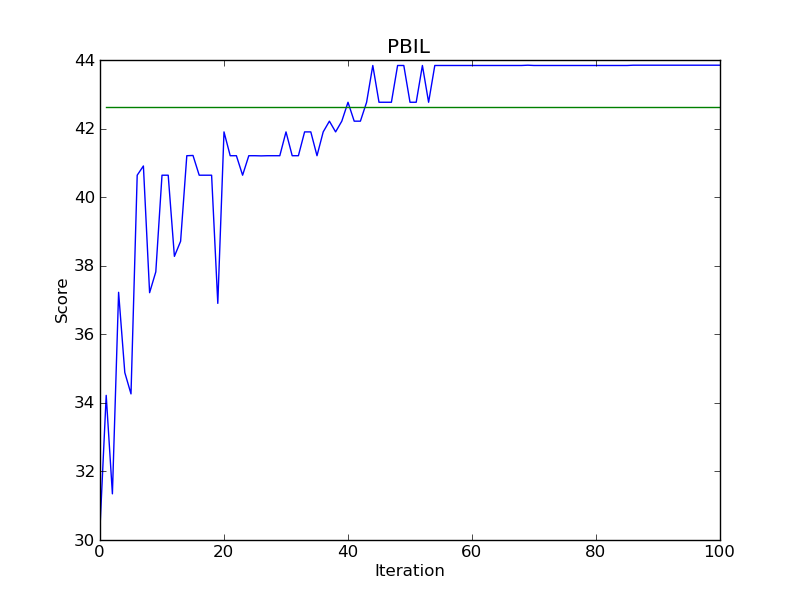
\includegraphics[width=10cm]{wykresy/matching_bids_100_goods_20_0000_txt_pbil.png}
    \caption{Wykres dla problemu 'matching' z 20 ofertami i 100 towarami.}
    \label{wyk:pbil1}
\end{figure}

\begin{figure}[!ht]
    \centering
    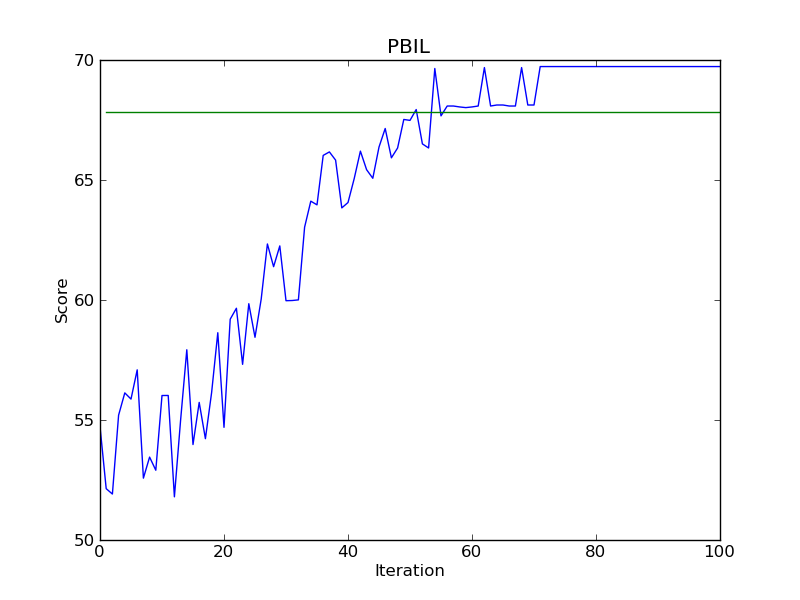
\includegraphics[width=10cm]{wykresy/matching_bids_100_goods_40_0000_txt_pbil.png}
    \caption{Wykres dla problemu 'matching' z 40 ofertami i 100 towarami.}
    \label{wyk:pbil2}
\end{figure}


\section{Rozwiązanie przy użyciu permutacji}
\subsection{Reprezentacja rozwiązania}
Rozwiązaniem problemu jest permutacja liczb naturalnych długości równej liczbie ofert.
Za oferty przyjęte jako zaakceptowane wybieramy zgodnie z kolejnością występowania w permutacji z pominięciem tych, których towary pokrywały się z towarami innej oferty występującej wcześniej.

\subsection{Funkcja celu}
Zgodnie z reprezentacją sumujemy ceny tych ofert, które zostały zaakceptowane. Przeglądamy permutacje od lewej do prawej i wybieramy te oferty, których towary nie zostały wykupione przez wcześniejsze oferty. Koszt obliczenia funkcji przystosowania dla jednego osobnika jest zatem taki sam jak w przypadku reprezentacji za pomocą wektora binarnego.

\subsection{Rozwiązanie}
Do rozwiązania tego problemu użyliśmy algorytmu SGA.
Jego parametry dobraliśmy ostatecznie na 200 iteracji i populację o rozmiarze 100 osobników.

\subsubsection{Krzyżowanie}
Do krzyżowania użyliśmy lekko zmodyfikowanego algorytmu PMX.
Założyliśmy, że funkcja celu zależy bardziej od elementów o mniejszym indeksie w permutacji niż większym.
Elementy o mniejszy indeksie są bardziej preferowane co wynika z funkcji celu, a oferty o dalszych indeksach mogą być często nie brane do rozwiązania ze względu na kolizje z wcześniejszymi ofertami.
Dlatego staramy się, aby wymieniamy przez operator PMX środkowy segment zaczynał się cześciej w niskich indeksach.


Wprowadzona modyfikacja polega na wyborze punktów $a$ i $b$ będących przedziałem wymienianego środkowego segmentu.
W pierwotnej wersji były losowane dwie liczby $x, y$ i na ich podstawie wyliczane punkty $a$, $b$.
\begin{equation}
    a = min(x, y) \cdot n \ \wedge \ b = max(x, y) \cdot n \ \ \hbox{gdzie n to długość permutacji}
\end{equation}
W zmodyfikowanej wersji punty były wyliczane w poniższy sposób.
\begin{equation}
    a = min(x, y)^2 \cdot n \ \wedge \ b = max(x, y) \cdot n
\end{equation}

\subsubsection{Mutacja}
Standardowe mutacje które stosowaliśmy w poprzednim projekcie okazały się mało skuteczne w zmienianiu wartości funkcji przystosowania. Wynikało to działania funkcji celu, które to powodowało, że często np. zamiana dwóch elementów w końcowej części permutacji miejscami nie zmieniała jej wartości.


Dodana przez nas mutacja jest dość prosta, ale okazała się znacząco poprawiać wyniki.
Polega na cyklicznym przesunięciu całej permutacji o jeden element w lewo.
W ten sposób oferta, która była pierwsza w permutacji staje się ostatnią.
Z zasady działania funkcji celu wiemy, że pierwsza oferta jest zawsze wybierana, a ostatnio dość rzadko dzięki czemu ta mutacja dość znacząco zmieniała osobniki.

\subsubsection{Wymiana}
Wymiana elementów polega na zastąpieniu najgorszych osobników stałą liczbą, ustawianą jako parametr, zmutowanych i skrzyżowanych osobników.
Dzięki odpowiednim doborze tej liczby populacja zawsze pamiętała stare najlepsze osobniki przez pewną liczbę iteracji co wpływało na poprawę znajdowanych wyników.

\subsubsection{Warunek stopu}
Na początku za warunek stopu przyjęliśmy unikalność wszystkich elementów.
Gdy wartości funkcji celu dla wszystkich elementów w populacji były takie same to przerywaliśmy algorytm.
Takie podejście okazało się jednak błędne, gdyż pomimo iż wartości funkcji celu były takie same to osobniki były znacząco różne w sensie permutacji i pozwolenie im na dalsze iteracje pozwalało poprawiać wyniki.

\subsection{Wyniki}
Wyniki przestawione są na wykresach (\ref{wyk:sga1}, \ref{wyk:sga2}, \ref{wyk:sga3}, \ref{wyk:sga4}).
Na niebiesko zaznaczono wynik dla algorytmu SGA dla kolejnych iteracji.
Na zielono zaznaczono najlepszy wynik algorytmu losowego, który wybierał wynik z takiej samej puli losowych osobników ile łącznie przegląda SGA.


Na wykresach \ref{wyk:sga1}, \ref{wyk:sga2} i \ref{wyk:sga3} algortym kończył swoje działanie gdy wszsytkie osobniki w populacji były unikalne pod względem wartości funkcji celu.
Na wykresie \ref{wyk:sga4} przestawiona jest wersja algorytmu, która kończyła poszukiwania  po ustalonej liczbie iteracji.
Podczas algorytmu próbowaliśmy również podmieniać niektóre stare osobniki nowymi losowymi gdy wszystkie poprzednie były już unikalne.
Jak widać takie podejście okazało się być lepsze od poprzedniego gdyż algorytm po pewnym czasie działania znajdował nieco lepsze rozwiązanie.


\begin{figure}[!ht]
    \centering
    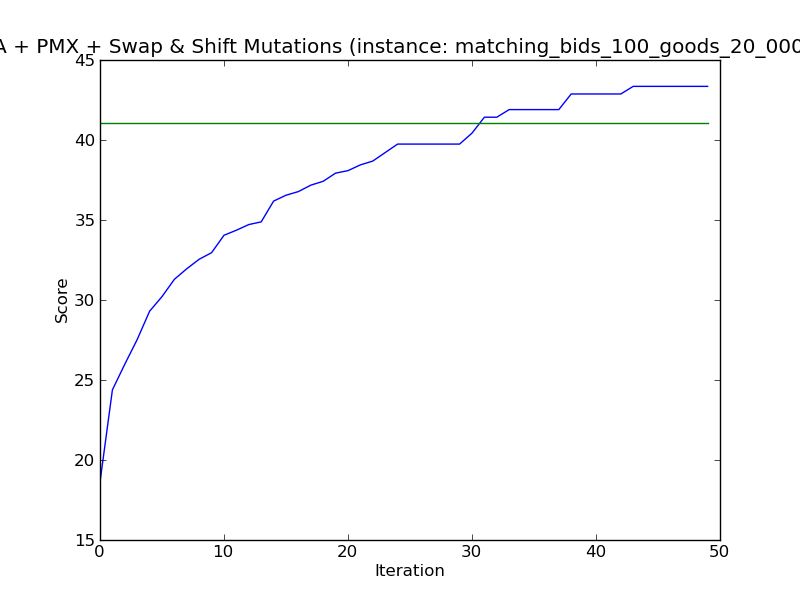
\includegraphics[width=10cm]{wykresy/matching_bids_100_goods_20_0000_txt_1.png}
    \caption{Wykres dla problemu 'matching' o parametrach 100 ofert i 20 towarów.}
    \label{wyk:sga1}
\end{figure}

\begin{figure}[!ht]
    \centering
    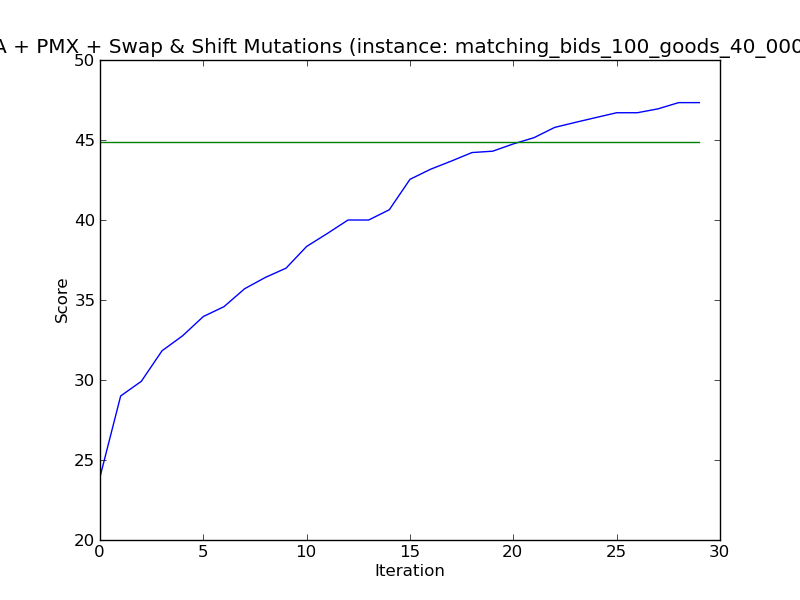
\includegraphics[width=10cm]{wykresy/matching_bids_100_goods_40_0000_txt_3.png}
    \caption{Wykres dla problemu 'matching' o parametrach 100 ofert i 40 towarów.}
    \label{wyk:sga2}
\end{figure}

\begin{figure}[!ht]
    \centering
    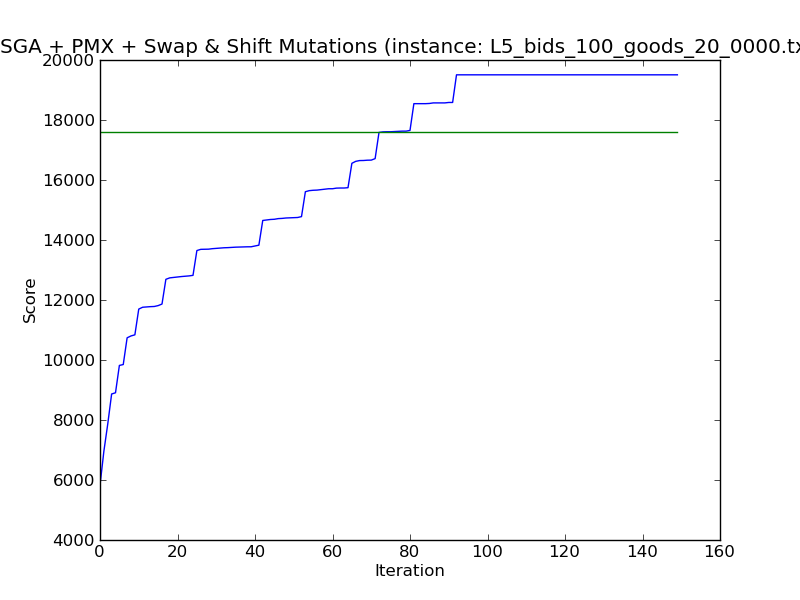
\includegraphics[width=10cm]{wykresy/L5_bids_100_goods_20_0000_txt_1.png}
    \caption{Wykres dla problemu 'L5' o parametrach 100 ofert i 20 towarów.}
    \label{wyk:sga3}
\end{figure}

\begin{figure}[!ht]
    \centering
    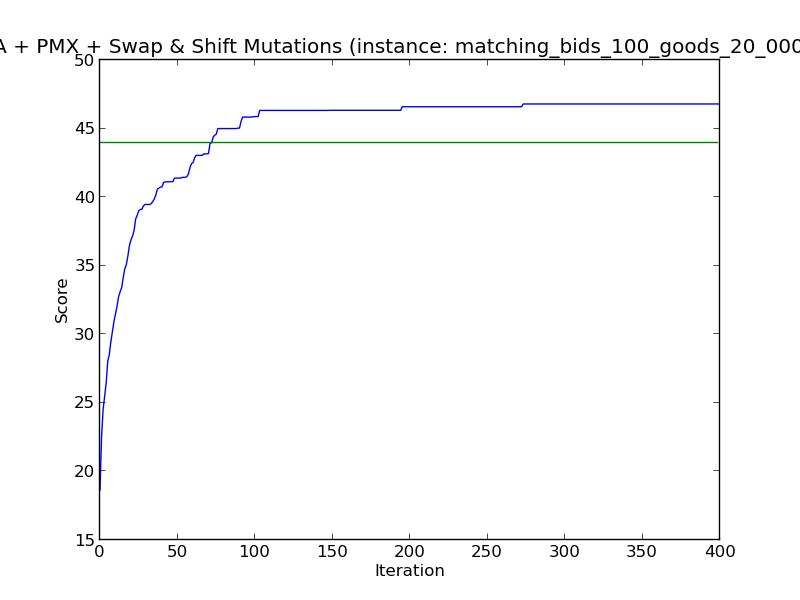
\includegraphics[width=10cm]{wykresy/matching_bids_100_goods_20_0000_txt_uniq.png}
    \caption{Wykres dla problemu 'matching' o parametrach 100 ofert i 20 towarów.}
    \label{wyk:sga4}
\end{figure}




\section{Porównanie}

\section{Podsumowanie}

\end{document}
